\section{Results} We compare binding site prediction results between two Geobind networks, one
without a CCRF layer (noCRF) and one with a CCRF layer as its second last layer (CRF). For both
cases we trained and validated the networks on three different datsets. The datasets used are as
follows:\\ \\ \textbf{PDNA-62 :} \citet{ahmad2004analysis} constructed a non-redundant dataset of 62
protein–DNA complexes which has been used in a variety of other studies
\citep{kuznetsov2006transient, wang2006bindn} etc. The protein sequences used were filtered to
ensure a maximum identity of no more than 25\% between any two sequences and the resolution of the
chosen structures was 2.5 A or better. The structures in this dataset contain only helical B-form
DNA.\\ \textbf{PDNA-74 :} We constructed a dataset of 74 single-stranded DNA binding proteins bound
to target ssDNA. We first used the structural database DNAproDB
\citep{sagendorf2017dnaprodb,sagendorf2020dnaprodb} to identify 374 protein-ssDNA complexes based on
structural critera which included ensuring the bound DNA in the structure presented the
single-stranded secondary structure, a minimum length of 4 nucleotides per DNA strand and 40
residues per protein chain, and a minimum of 5 nucleotide-residue interactions (as defined by
DNAproDB). Next, we verified that all proteins identified had known ssDNA binding function based on
annotations from the Gene Ontology knowledgebase \citep{gene2019gene}.  Finally, all protein
sequences were clustered with a 70\% sequence identity threshold using CD-HIT \citep{li2006cd}.
These clusters were then randomly sampled, with up to three samples per cluster, to generate the
final set of 74 protein structures. This sampling method allows us to construct a dataset with
limited amount of sequence redundancy but more conformational sampling than would be possible with a
stricter requirement on sequence redundancy. This is useful in the case of ssDNA where the polymer
is very flexible, but structural data is limited.\\ \textbf{PDNA-224:} a non-redundant dataset of
224 protein-DNA complexes originally constructed by \citet{li2013predna}\\ \begin{center}
        \begin{figure}
                \makebox[\textwidth]{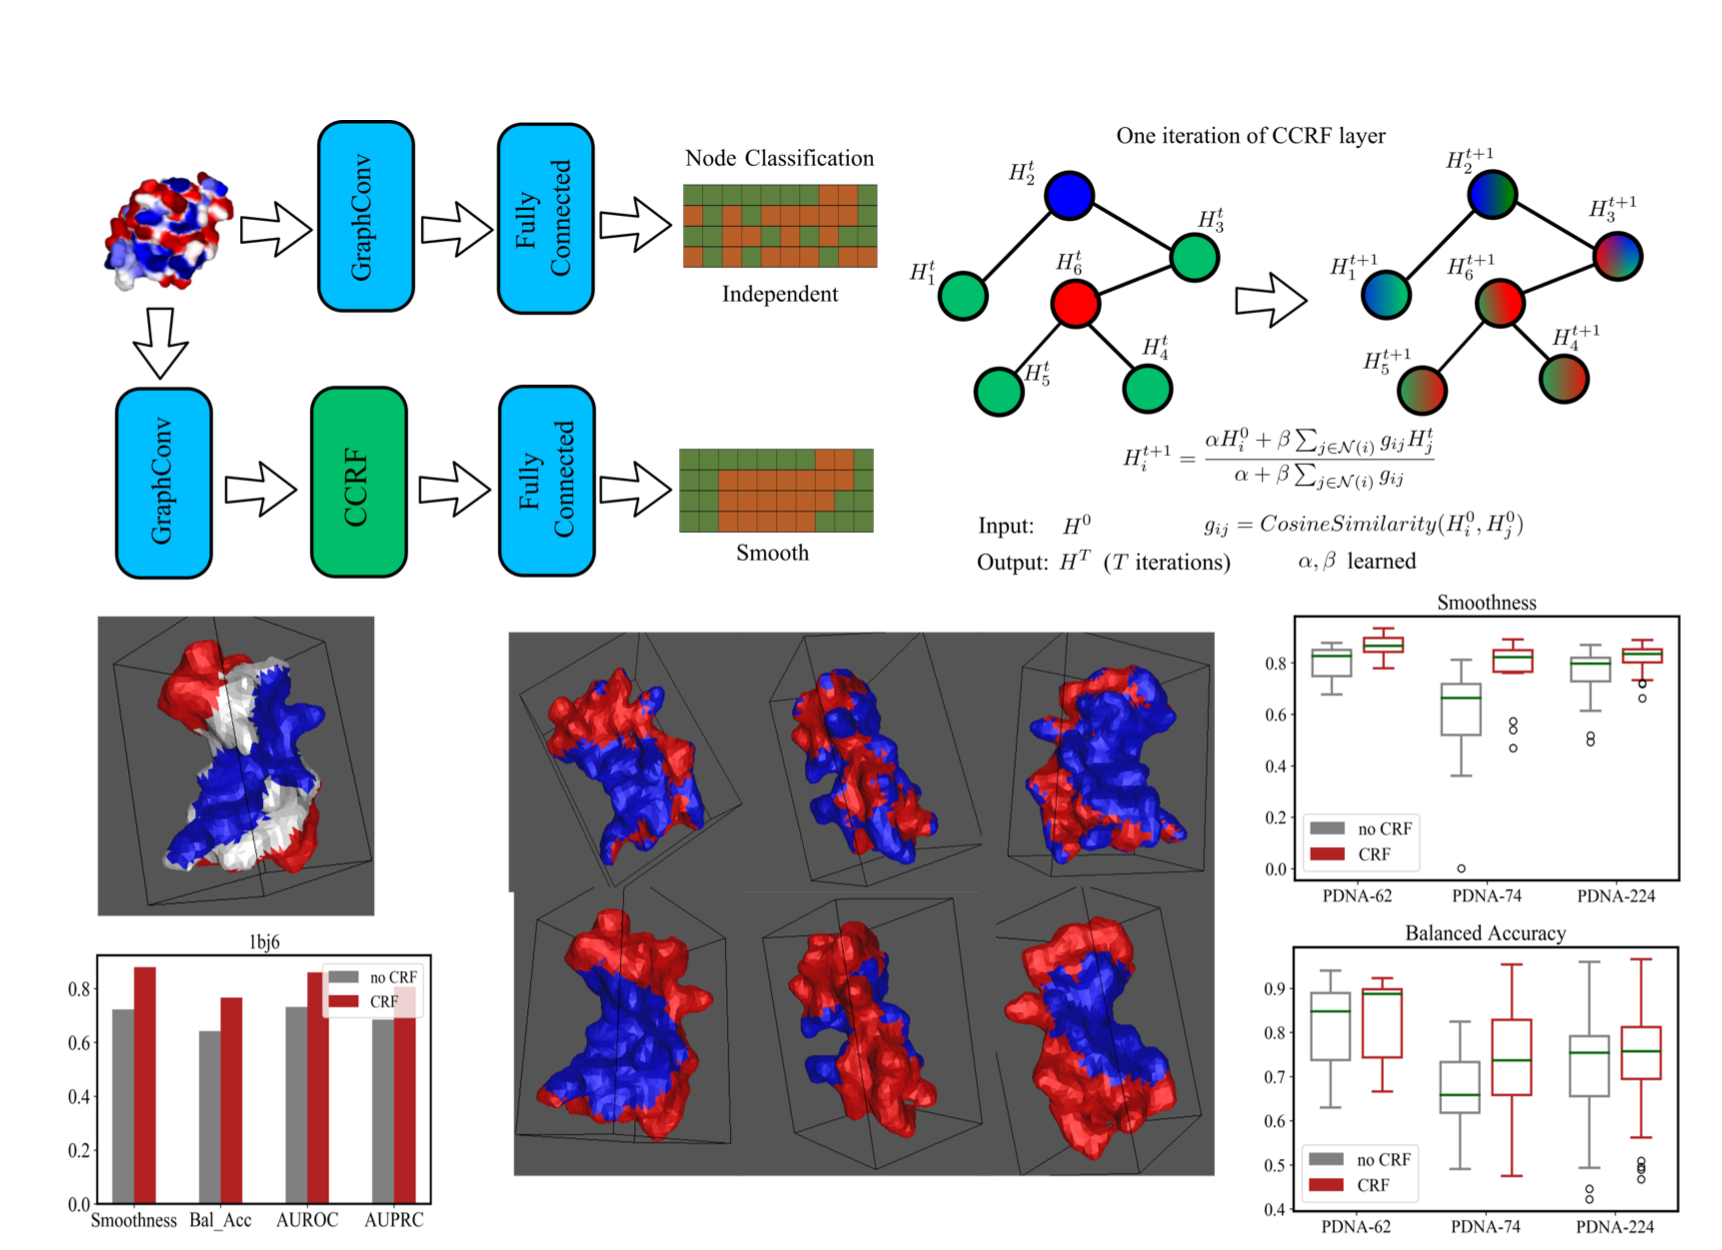
\includegraphics[width=0.8\paperwidth]{crf_figs/demo_crf_fig.png}}
 % archetecture.png: 1149x508 px, 72dpi, 40.53x17.92 cm, bb=0 0 1149 508
        \caption[CCRF for smooth binding site label prediction over protein surface.]{\textbf{CCRF
        for smooth binding site label prediction over protein surface.} ({\bf A}) ({\bf B}) }
        \label{fig:ccrf} \end{figure} \end{center}

Both CRF and noCRF models were trained on the three datasets with a 4:1 training and validation set
        split. \red{\hyperref[fig:ccrf]{Fig. 2.3}} shows smoothness( eq.
        \ref{final_smoothness_metric}) and Balanced Accuracy  metrics achieved on the validation set
        in each case. We can clearly the smoothness of the predictions have increased significantly.
        It should also be noted that that, median Balanced Acuracy has also increased for all three
        cases. Therefore, we can conclude applying the CCRF layer improves the smoothness of the
        predicted labels over mesh vertices without compromizing in accuracy of prediction. For a
        more visual understanding, \red{\hyperref[fig:ccrf]{Fig. 2.1C}} shows one particular example
        of the effect of using CRF layer against the noCRF model for a protein in the validation set
        for PDNA-74 dataset. The top left panel in \red{\hyperref[fig:ccrf]{Fig. 2.1C}} shows the
        ground truth data. We can clearly see how the CRF model improves smoothness of the
        prediction along with various other classification metrics.


